\providecommand{\main}{..} 
\documentclass[\main/boa.tex]{subfiles}

\begin{document}

\section{Jak dużo mocy (i po co) można wycisnąć z modelu predykcyjnego?}


\begin{minipage}{0.915\textwidth}
	\centering
  {\bf \LARGE \index[a]{Suchwałko Artur} Artur Suchwałko}
\end{minipage}


\begin{affiliations}
\begin{minipage}{0.915\textwidth}
\centering
\large QuantUp \\[1pt]
Kontakt: \href{mailto:artur@quantup.pl}{\nolinkurl{artur@quantup.pl}}\\
\end{minipage}
\end{affiliations}


W modelowaniu predykcyjnym często wybieramy bardzo złożone podejścia i modele. Z~drugiej strony, często też stosuje się podejścia do modelowania, które wręcz jest wstyd stosować w dzisiejszych czasach.

Predykcję można poprawić na różne sposoby, na przykład poprzez wykorzystanie bardziej złożonych modeli, staranny dobór hiperparametrów, uwzględnienie kosztów błędnej klasyfikacji czy zmianę kryterium optymalizacji.

Pokażę na przykładzie, co to daje dla biznesu oraz jak to zrobić w R.

\bio
\begin{wrapfigure}{r}{100px}
    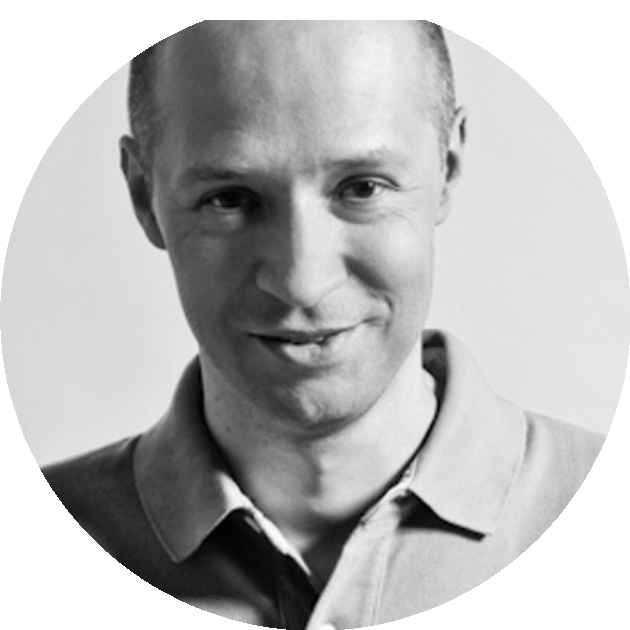
\includegraphics[width=100px]{img/guests/czarno_biale/artur.png}
\end{wrapfigure} 
Artur Suchwałko ma dwudziestoletnie doświadczenie w projektach analitycznych. Pracował dla różnych firm, od start-upów po międzynarodowe korporacje i w różnych rolach, od pracownika, przez konsultanta, po właściciela. Jest doświadczonym programistą oraz menedżerem projektów. Przez kilkanaście lat pracy statystyka w~banku zajmował się głównie budową modeli predykcyjnych i~tworzeniem oprogramowania do ich budowy. W tym samym czasie został doktorem matematyki i napisał kilkanaście prac naukowych. Od pięciu lat rozwija z sukcesem swoją firmę QuantUp, zajmującą się analizą danych, modelowaniem statystycznym i tworzeniem oprogramowania oraz szkoleniami z tych dziedzin.

Przeprowadził przynajmniej kilkadziesiąt projektów i kilka tysięcy godzin komercyjnych szkoleń z głębszej analityki biznesowej. Jest współwłaścicielem, Vice CEO i CSO szwedzkiej firmy bioinformatycznej MedicWave. Od kilkunastu lat wykorzystuje w biznesie darmowe \break oprogramowanie (głównie R) i promuje jego używanie. Jest fanem R i współautorem wydanej w PWN książki o prognozowaniu w R.

\end{document}
